% Overview figure for the neural error mitigation framework.
% Standalone TikZ document; compile with pdflatex.
\documentclass[tikz,border=8pt]{standalone}
\usepackage{amsmath,amssymb}
\usetikzlibrary{positioning,calc,arrows.meta,backgrounds}

% ---- Muted, colorblind-safe palette (Okabe--Ito tints) ----
\definecolor{qblue}{RGB}{62,105,150}
\definecolor{qblueLight}{RGB}{224,236,246}
\definecolor{qorange}{RGB}{186,116,42}
\definecolor{qorangeLight}{RGB}{253,236,214}
\definecolor{qgreen}{RGB}{47,122,91}
\definecolor{qgreenLight}{RGB}{224,240,231}
\definecolor{qred}{RGB}{172,82,54}
\definecolor{qredLight}{RGB}{251,230,222}
\definecolor{qgray}{RGB}{105,108,112}
\definecolor{qgrayLight}{RGB}{241,242,244}

\begin{document}
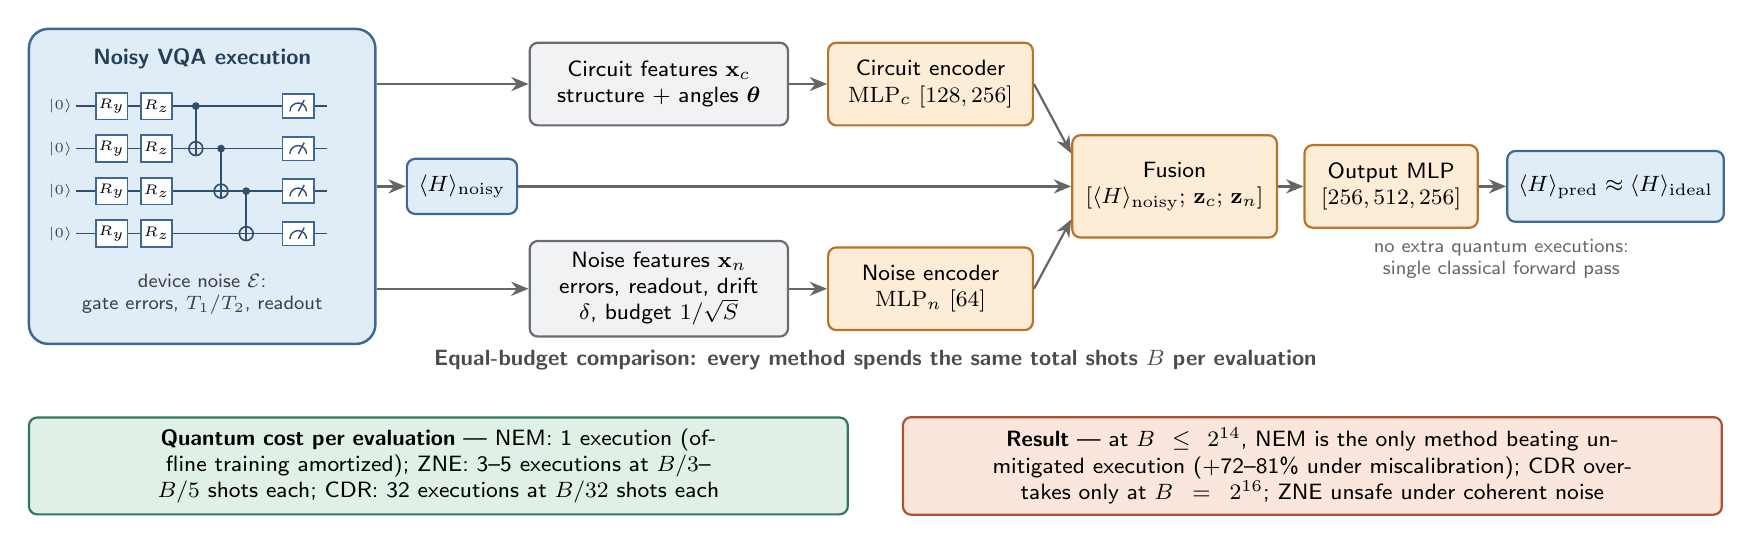
\begin{tikzpicture}[
    font=\sffamily\small,
    qbox/.style={rectangle, rounded corners=3pt, draw, line width=0.8pt,
                 align=center, font=\sffamily\footnotesize, inner sep=4pt},
    bluebox/.style={qbox, draw=qblue, fill=qblueLight},
    graybox/.style={qbox, draw=qgray, fill=qgrayLight},
    orangebox/.style={qbox, draw=qorange, fill=qorangeLight},
    greenbox/.style={qbox, draw=qgreen, fill=qgreenLight},
    redbox/.style={qbox, draw=qred, fill=qredLight},
    panel/.style={rectangle, rounded corners=7pt, draw=qblue, fill=qblueLight,
                  line width=0.9pt},
    gate/.style={rectangle, draw=qblue, fill=white, inner sep=1pt,
                 minimum size=0.34cm, font=\tiny, line width=0.6pt},
    wire/.style={draw=qblue!75!black, line width=0.6pt},
    arrow/.style={-{Stealth[length=2.2mm, width=1.8mm]}, line width=0.8pt,
                  draw=black!60, rounded corners=4pt},
]

% =====================================================================
% (a) Left panel: noisy VQA execution on a 4-qubit hardware-efficient
%     ansatz (RY/RZ rotation layer + linear CX chain + measurement)
% =====================================================================
\node[panel, minimum width=4.4cm, minimum height=4.0cm] (vqa) at (2.2, 2.3) {};
\node[font=\sffamily\footnotesize\bfseries, text=qblue!60!black] at (2.2, 3.92)
    {Noisy VQA execution};

% qubit wires
\foreach \y in {3.32, 2.78, 2.24, 1.70} {
    \node[font=\tiny, text=black!75] at (0.40, \y) {$|0\rangle$};
    \draw[wire] (0.60, \y) -- (3.78, \y);
}

% rotation layer: RY then RZ
\foreach \y in {3.32, 2.78, 2.24, 1.70} {
    \node[gate] at (1.05, \y) {$R_y$};
    \node[gate] at (1.62, \y) {$R_z$};
}

% linear CX entanglement chain (control dot -> target circle-plus)
\newcommand{\cnot}[3]{% x, y_control, y_target
    \fill[qblue!75!black] (#1, #2) circle (1.4pt);
    \draw[qblue!75!black, line width=0.6pt] (#1, #3) circle (2.5pt);
    \draw[qblue!75!black, line width=0.6pt] (#1, #2) -- ($(#1, #3)+(0,-2.5pt)$);
    \draw[qblue!75!black, line width=0.6pt]
        ($(#1, #3)+(-2.5pt,0)$) -- ($(#1, #3)+(2.5pt,0)$);
}
\cnot{2.12}{3.32}{2.78}
\cnot{2.44}{2.78}{2.24}
\cnot{2.76}{2.24}{1.70}

% measurement meters
\foreach \y in {3.32, 2.78, 2.24, 1.70} {
    \node[gate, minimum width=0.40cm, minimum height=0.30cm] at (3.42, \y) {};
    \draw[qblue!75!black, line width=0.5pt]
        ($(3.42, \y)+(-3.0pt,-1.9pt)$) arc[start angle=180, end angle=0, radius=3.0pt];
    \draw[qblue!75!black, line width=0.5pt] ($(3.42, \y)+(0,-1.9pt)$) -- ++(62:4.6pt);
}

% device-noise annotation inside the panel
\node[font=\sffamily\scriptsize, text=black!75, align=center] at (2.2, 0.93)
    {device noise $\mathcal{E}$:\\ gate errors, $T_1/T_2$, readout};

% noisy expectation value
\node[bluebox, minimum width=1.4cm, minimum height=0.7cm] (hnoisy) at (5.5, 2.3)
    {$\langle H \rangle_{\mathrm{noisy}}$};
\draw[arrow] (vqa.east) -- (hnoisy.west);

% =====================================================================
% (b) Two parallel feature branches
% =====================================================================
\node[graybox, text width=3.0cm, minimum width=3.2cm, minimum height=1.05cm] (xc) at (8.0, 3.6)
    {Circuit features $\mathbf{x}_c$\\ structure $+$ angles $\boldsymbol{\theta}$};
\node[graybox, text width=3.0cm, minimum width=3.2cm, minimum height=1.05cm] (xn) at (8.0, 1.0)
    {Noise features $\mathbf{x}_n$\\ errors, readout, drift $\delta$, budget $1/\sqrt{S}$};

\node[orangebox, minimum width=2.6cm, minimum height=1.05cm] (mlpc) at (11.45, 3.6)
    {Circuit encoder\\ $\mathrm{MLP}_c$ $[128, 256]$};
\node[orangebox, minimum width=2.6cm, minimum height=1.05cm] (mlpn) at (11.45, 1.0)
    {Noise encoder\\ $\mathrm{MLP}_n$ $[64]$};

\draw[arrow] (vqa.east |- xc) -- (xc.west);
\draw[arrow] (vqa.east |- xn) -- (xn.west);
\draw[arrow] (xc.east) -- (mlpc.west);
\draw[arrow] (xn.east) -- (mlpn.west);

% =====================================================================
% (c) Fusion and prediction
% =====================================================================
\node[orangebox, minimum width=2.6cm, minimum height=1.3cm] (fusion) at (14.55, 2.3)
    {Fusion\\ $[\langle H \rangle_{\mathrm{noisy}};\, \mathbf{z}_c;\, \mathbf{z}_n]$};
\node[orangebox, minimum width=2.2cm, minimum height=1.05cm] (outmlp) at (17.3, 2.3)
    {Output MLP\\ $[256, 512, 256]$};
\node[bluebox, minimum width=2.7cm, minimum height=0.9cm] (pred) at (20.15, 2.3)
    {$\langle H \rangle_{\mathrm{pred}} \approx \langle H \rangle_{\mathrm{ideal}}$};

% embeddings converge into the fusion block (straight arrows)
\draw[arrow] (mlpc.east) -- ($(fusion.west)+(0, 0.42)$);
\draw[arrow] (mlpn.east) -- ($(fusion.west)+(0,-0.42)$);

% noisy value feeds the fusion directly (clear corridor between branches)
\draw[arrow] (hnoisy.east) -- (fusion.west);

\draw[arrow] (fusion.east) -- (outmlp.west);
\draw[arrow] (outmlp.east) -- (pred.west);

% lightweight-inference note
\node[font=\sffamily\scriptsize, text=black!60, align=center] at (18.7, 1.38)
    {no extra quantum executions:\\ single classical forward pass};

% =====================================================================
% (d) Complementarity strip
% =====================================================================
\node[font=\sffamily\footnotesize\bfseries, text=black!70] at (10.75, 0.10)
    {Equal-budget comparison: every method spends the same total shots $B$ per evaluation};

\node[greenbox, text width=9.7cm, minimum width=10.4cm, minimum height=1.1cm]
     (regA) at (5.2, -1.25)
    {\textbf{Quantum cost per evaluation} --- NEM: 1 execution (offline training amortized);
     ZNE: 3--5 executions at $B/3$--$B/5$ shots each; CDR: 32 executions at $B/32$ shots each};
\node[redbox, text width=9.7cm, minimum width=10.4cm, minimum height=1.1cm]
     (regB) at (16.3, -1.25)
    {\textbf{Result} --- at $B \le 2^{14}$, NEM is the only method beating unmitigated execution
     (+72--81\% under miscalibration); CDR overtakes only at $B = 2^{16}$;
     ZNE unsafe under coherent noise};

\end{tikzpicture}
\end{document}
